\documentclass[14pt]{extarticle}
\usepackage[
left=30mm,
top=20mm,
right=15mm,
bottom=20mm,
]{geometry}

\usepackage{graphicx}
\usepackage[utf8x]{inputenc}
\usepackage[russian]{babel}
\usepackage[T1]{fontenc}
\usepackage{float}
\usepackage{listings}
\usepackage{cite}
\usepackage{hyperref}
\usepackage{etoolbox}
\usepackage{indentfirst}
\usepackage[linesnumbered,boxed]{algorithm2e}
\sloppy

\graphicspath{{Figures//}}%путь к рисункам


\lstset{inputencoding=utf8x, extendedchars=false, keepspaces = true,
language=C++,
keywords={include, const, virtual, template, typename, class, private, public, operator, if, while, else, return, new, delete, int, float, bool, char},
sensitive=true,
%basicstyle=\small,
commentstyle=\scriptsize\rmfamily,
keywordstyle=\ttfamily\underbar,
identifierstyle=\ttfamily,
basewidth={0.5em,0.5em},
columns=fixed,
fontadjust=true,
breaklines=true,
literate={->}{{$\to$}}1
}

\makeatletter
\renewcommand{\@biblabel}[1]{#1.} % Заменяем библиографию с квадратных скобок на точку:
\makeatother
\gappto\captionsrussian{\renewcommand{\contentsname}{Оглавление}}
\renewcommand\baselinestretch{1.5}
\renewcommand{\lstlistingname}{Результат}

\begin{document}

\begin{titlepage}
\thispagestyle{empty}
\def\baselinestretch{1.0}
\begin{center}
	{САНКТ-ПЕТЕРБУРГСКИЙ ГОСУДАРСТВЕННЫЙ УНИВЕРСИТЕТ \\ \vskip 0.3em {\large Математико-механический факультет \\ \vskip 0.7em{\large Кафедра информатики \\}}}
    \vspace*{0.15\textheight}
    {\large Крень Мария}
    
    \vskip 2em
    {\huge Пользовательский уровень библиотеки неконсервативной сборки мусора для C++}
    
    \vskip 1em
    {\large Дипломная работа} \\
    \vskip 2em
    {\normalsize \raggedleft 
    Допущена к защите.\\
    Зав. кафедрой:\\
    д.ф.-м.н., Н.К.Косовский 
    \\[3em]
    Научный руководитель:\\
    к.ф.-м.н. Д.Ю.Булычев
    \\[3em]
    Рецензент:\\
    к.ф.-м.н. Д.В.Кознов\\
    \vspace*{0.08\textheight}
    {\centering Санкт-Петербург \\ 2014}
    }
\end{center}
\end{titlepage}
\begin{titlepage}
\thispagestyle{empty}
\def\baselinestretch{1.0}
\begin{center}
	{\large SAINT-PETERSBURG STATE UNIVERSITY \\ \vskip 0.3em {\large Mathematics and Mechanics Faculty \\ \vskip 0.7em{\large Informatics Chair \\}}}
    \vspace*{0.15\textheight}
    {\large Mariya Kren}
    
    \vskip 2em
    {\huge User Level of a Non-Conservative Garbage Collection Library for C++}
    
    \vskip 1em
    {\large Graduation Thesis} \\
    \vskip 2em
    {\normalsize \raggedleft 
    Admitted for defence.\\
    Head of the chair:\\
    professor N.K. Kosovsky
    \\[3em]
    Scientific supervisor:\\
    Dr. D.Yu. Boulytchev
    \\[3em]
    Reviewer:\\
    Dr. D.V.Koznov\\
    \vspace*{0.08\textheight}
    {\centering Saint-Petersburg \\ 2014}
    }
\end{center}
\end{titlepage}
\tableofcontents
\thispagestyle{empty} 
\section*{Введение}

Ручное управление памятью в языках, подобных C++, является источником большого количества трудно отслеживаемых ошибок, наличия которых можно было бы
избежать, сделав процесс управления памятью автоматическим. \textit{Сборка мусора} является одним из способов автоматического управления памятью, при
котором освобождение памяти выводится из-под контроля ПО на прикладном уровне. При автоматическом управлении программист не может явно влиять на распределение
объектов в памяти, у него есть лишь
косвенные способы сделать это с помощью использования тех или иных языковых конструкций. В идеальном случае, для рационального использования
памяти необходимо освобождать память, занимаемую объектами, которые более не будут использованы программой. Поскольку точно определить, что
объект не будет использован в дальнейшем, невозможно, на практике используют критерий доступности. \textit{Доступность} --- это консервативное
приближение используемости. \textit{Мусором}, в таком случае, называют объект, все пути доступа к которому уже разрушены, а память из-под него
ещё не освобождена. В некоторое, заранее определенное время, например, в простейшем случае, когда перестаёт хватать свободной памяти, выполнение
программы временно приостанавливается и запускается процесс \textit{сборки мусора}, который освобождает всю или ту, что возможно, память,
занятую мусором, после чего управление возвращается обратно программе. \textit{Сборщиком мусора} называется компонент, производящий \textit{сборку мусора}.

Процесс \textit{сборки мусора}, в простейшем случае, делят на три этапа:
\begin{enumerate}
\item \textit{Построение корневого множества}. На этом этапе строится множество объектов, которые считаются изначально доступными.
Такие объекты называются \textit{корнями} (англ. roots). Данное построение
аксиоматично, т.е. основывается на некотором наборе правил, согласно которым те или иные элементы считаются доступными. Данный этап является неотъемлемой
частью любого сборщика мусора.
\item \textit{Маркировка}. Начиная с множества, построенного на предыдущем этапе, происходит сканирование памяти, и все объекты, до которых возможно
добраться из построенного корневого множества, считаются доступными; оставшиеся объекты считаются мусором.
\item \textit{Освобождение}. Происходит сканирование кучи, в течение которого память из-под всех элементов, помеченных как мусор или не отмеченных как
доступные, освобождается.
\end{enumerate}

Есть несколько требований, которые должны быть выполнены для реализации сборки мусора:
\begin{enumerate}
\item Возможность построения корневого множества. Иными словами, необходимо иметь возможность идентифицировать все указатели в программном стеке, регистрах
и статической области памяти.
\item Должна присутствовать возможность определить все указатели из любого объекта на другие элементы кучи.
\end{enumerate}
В таких языках, как LISP или JAVA все условия соблюдаются, и в них успешно используется технология сборки мусора, в то время как, например,
в языке C не все условия выполняются. В языках, где не соблюдаются хотя бы одно из вышеперечисленных условий, возможна исключительна
\textit{консервативная сборка мусора}.
\textit{Консервативной} называется такая сборка мусора, при которой любой элемент данных, значение которого может быть истолковано, как указатель на
некоторый элемент кучи, считается  таковым. Консервативный подход к сборке мусора не позволяет собрать весь мусор, что может стать проблемой при обработке
большого количества данных. Неконсервативная сборка мусора лишена подобного недостатка и способна освободить всю память программы, более не
являющуюся доступной. \textit{Неконсервативным} или  \textit{точным сборком мусора} называется сборщик мусора, имеющий возможность точно распознать
все указатели в памяти. Иными словами, точный сборщик мусора --- это сборщик мусора, не использующий консервативный подход.

В C++ не соблюдаются требования, необходимые для сборки сборки мусора, реализовать точный сборщик мусора без ограничений
на использование некоторых примитивов языка не представляется возможным.
Более того, в C++ имеется ряд технических сложностей, затрудняющих реализацию точного сборщика мусора.
Тем не менее, в случае соблюдения программистом некоторых соглашений на програмный код,
точная сборка мусора становится возможной и в C++.

Целями работы является реализация основных примитивов библиотеки неконсервативной сборки мусора для C++,
обеспечение возможности совмещения ручного и автоматического управления памятью.
\newpage
\section{Постановка задачи}

Целью данной работы является создание пользовательского уровня для библиотеки неконсервативной сборки 
мусора для С++. Следующие основные подзадачи были выделены для её достижения:

\begin{itemize}
\item изучить и проанализировать существующие подходы к автоматизации управлением памятью 
для языка С++;

\item предложить и реализовать собственное решение на основе проведенного анализа;

\item продемонстрировать работоспособность реализованного сборщика мусора.
\end{itemize}

\newpage
\section{Некоторые средства автоматизации\\
управления памятью для С++}

Одним из наиболее широко используемых средств автоматизации управления памятью в
контексте языка С++ являются ``умные указатели'' (smart pointers). ``Умный указатель''~---
это специальный объект, который хранит указатель на участок динамически отведенной области
памяти и определяет некоторую дисциплину обращения с этом указателем. Иногда следование
этой дисциплине является лишь соглашением, и тогда ``умный указатель'' является всего лишь
способом идентифицировать необходимость правильного обращения с данными; однако довольно часто
``умные указатели'' действительно определенным образом ограничивают набор возможных
способов манипулирования данными за счет использования декларативных возможностей языка С++.

Простейший ``умный указатель'' может выглядеть так:

\begin{lstlisting}
    template <typename T> class smart_pointer {
      T *m_obj; // Указатель на динамические данные
      public:
        // Конструктор получает исходный указатель 
        smart_pointer (T *obj) : m_obj(obj) {}
        // Деструктор удаляет адресуемые данные
        ~smart_pointer () { delete m_obj; }
        // Перегруженные операторы для обращения к данным
        T* operator-> () { return m_obj; }
        T& operator*  () { return *m_obj; }
    }
\end{lstlisting}

Такой указатель позволяет обеспечить автоматическое освобождение области динамической памяти, если 
время её жизни можно ограничить временем жизни самого ``умного указателя''. При этом никак не
контролируется, что сам ``умный указатель'' используется правильно --- например, что конструктор
получает действительно адрес в куче или что для данного адреса создан только один ``умный указатель''.

Другим примером ``умного указателя''является \lstinline{Boost::scoped_ptr}\footnote{\url{http://www.boost.org/doc/libs/1_39_0/libs/smart_ptr/scoped_ptr.htm}} 
библиотеки BOOST\footnote{\url{http://www.boost.org}}. Его основное отличие от приведенного выше~--- отсутствие возможности копирования и присваивания (а,
значит, и передачи параметром в функцию). Эти ограничения не исключают возможность неправильного использования, но позволяют избежать некоторых из них.

Еще одним вариантом является \lstinline{auto_ptr}\footnote{\url{http://www.cplusplus.com/reference/memory/auto_ptr}}. Этот указатель разрешает
операции копирования и передачи параметром, но при этом ``опустошается'' содержимое источника. Таким образом, указатели не копируются, 
а ``перемещаются'', что позволяет избежать ситуации, когда происходит несколько попыток освободить одну и ту же область памяти из-за хранения 
её адреса разными ``умными указателями''. С другой стороны, теперь не гарантируется, что ``умный указатель'' всегда указывает на правильные данные ---
в какой-то момент он может ``испортиться''. В силу этого такие указатели нельзя использовать в контейнерах STL. Для таких целей используются
\lstinline{std::shared_ptr}.

\lstinline{shared_ptr}\footnote{\url{http://www.cplusplus.com/reference/memory/shared_ptr}}~--- это ``умный указатель'' с подсчетом ссылок. Это значит, 
что с каждой областью памяти, адресуемой \lstinline{shared_ptr}, ассоциирована переменная, которая хранит количество указателей, которые ссылаются на начало
этой области памяти. Если эта переменная становится равной нулю, то область освобождается. Счетчик инкрементируется при каждом вызове оператора копирования 
или оператора присваивания. У \lstinline{shared_ptr} есть оператор приведения к типу \lstinline{bool}, что позволяет проверять, указывает ли он на что-нибудь.
Использование \lstinline{shared_ptr} может обеспечить сравнительно безопасную автоматизацию управления памятью, однако неприятности все же возможны. Во-первых,
наличие указателя \lstinline{shared_ptr} не на начало динамически отведенной области памяти не гарантирует её сохранения; кроме того, циклические
ссылки приводят к образованию неудаляемого мусора; наконец, возможна ситуация лавинообразного освобождения памяти с возникновением непредсказуемой
задержки.

\newpage
\section{Используемые особенности языка С++}

Реализация сборки мусора в виде внешней библиотеки существенно опирается 
на некоторые особенности как языка С++, так и его компиляторов и среды поддержки времени 
исполнения. К таковым особенностям относятся:

\begin{enumerate}
\item функция \lstinline{typeid} и возможность идентификации типа во время исполнения (runtime type identification, RTTI);
\item инициализация по размещению (placement new);
\item шаблоны, в том числе шаблоны с переменным числом аргументов (templates, variadic templates);
\item конструкторы, деструкторы и порядок их вызова.
\end{enumerate}

Далее рассмотрим вышеперечисленные особенности подробнее.

\subsection{Функция \lstinline{typeid} и идентификация типа\\
во время исполнения} 

Идентификация типа во время исполнения позволяет получить метаинформацию о типе объекта во время работы программы. 
В сборщике мусора эта метаинформация используется для установления связи между объектом и метаинформацией сборщика
мусора, соответствующей этому типу. Для того, чтобы это стало возможно, поддержка RTTI должна быть включена 
соответствующими опциями компилятора.

На пользовательском уровне возможности RTTI представлены функцией \lstinline{typeid}\footnote{\url{http://www.c-cpp.ru/books/identifikaciya-tipa-vo-vremya-ispolneniya-rtti}},
которая получает указатель на объект и возвращает ссылку на объект типа \lstinline{typeinfo}. Данный тип
содержит информацию о типе объекта, в частности, имя этого типа, которое и используется в сборщике мусора.

\subsection{Инициализация по размещению, шаблоны,\\
шаблоны с произвольным числом аргументов} 

Инициализация по размещению и шаблоны с произвольным числом аргументов в реализации сборщика мусора используются 
совместно для того, чтобы выразить примитив выделения памяти. Основная задача, которая при этом возникает 
кроме собственно выделения~--- определение типа объекта, занимающего данную область памяти, и её аннотирование
соответствующей метаинформацией. 

Отследить момент выделения памяти можно было бы путем перегрузки глобального оператора \lstinline{new}; однако
в этом случае было бы трудно узнать, каков тип объекта, для которого выделяется память. Использование же
инициализации по размещению, шаблонов и шаблонов с произвольным числом аргументов позволяет инкапсулировать
всю нужную функциональность в одной функции, которая отведет память, вызовет конструктор, передав
ему нужное количество аргументов, и кроме того выполнит все остальные необходимые действия.

 \subsection{Конструкторы, деструкторы и порядок их вызова} 

Важным фактом является то, что в С++ момент создания/удаления объекта можно отследить с помощью 
конструктора/деструктора\footnote{\url{http://www.developerfusion.com/article/133063/constructors-in-c11/}}. 
В сборщике мусора это используется для того, чтобы, во-первых, построить метаинформацию для данного типа (каждый
``умный указатель'' при создании регистрирует себя в некоторой структуре данных) и, во-вторых, чтобы регистрировать
корневые указатели во внешнем пуле корней.

\newpage
\section {Пользовательский уровень библиотеки\\
сборки мусора}

С точки зрения пользователя библиотека сборки мусора представлена одним шаблонным классом
``умного указателя'' 

\begin{lstlisting}
    template <class T> class gc_ptr {
       ...
    }
\end{lstlisting}

и одной шаблонной функцией выделения памяти

\begin{lstlisting}
    template <class T, typename ... Types> T* gc_new (
    Types ... types, size_t count = 1
    ) {
       ...
    }
\end{lstlisting}

которые становятся доступными после подключения одного заголовочного файла:

\begin{lstlisting}
    # include <libgc/libgc.h>
\end{lstlisting}

Исполняемый код библиотеки содержится в модулях, которые могут быть как собраны статически вместе
с приложением, так и подгружены динамически.

Любая программа, которая в качестве примитива выделения памяти использует \lstinline{gc_new}, в качестве
указателей --- \lstinline{gc_ptr}, и не содержит явного освобождения памяти с помощью \lstinline{delete}, будет
работать с использованием сборки мусора.

Семантика описанных примитивов с точки зрения сборки мусора будет описана в следующем разделе; пока же
мы обсудим их интерфейс с точки зрения пользователя.

\subsection{Интерфейс \lstinline{gc_ptr}}

Класс \lstinline{gc_ptr} инкапсулирует всю функциональность указателя, которая безопасна с точки зрения
сборки мусора. Данный класс реализует следующие операторы:

\begin{enumerate}
\item \lstinline{T& operator*() const}~--- разыменование;
\item \lstinline{T* operator->() const, operator T* () const}~--- доступ к указателю;
\item \lstinline{T& operator[](size_t index)}~--- доступ к элементам массива;
\item \lstinline{bool operator== (const gc_ptr <T> &a), bool operator== (const T* a)}~--- проверки на равенство;
\item \lstinline{bool operator!= (const gc_ptr <T> &a), bool operator!= (const T* a)}~--- проверки на неравенство;
\item \lstinline{gc_ptr& operator = (const gc_ptr <T> &a), gc_ptr& operator = (T* a)}~--- присваивание.
\end{enumerate}

Кроме того, у данного класса два конструктора: \lstinline{gc_ptr (T* p)} и \lstinline{gc_ptr (const gc_ptr <T> &p)}. 

\subsection{Функция выделения памяти \lstinline{gc_new}}

В языке С++ существует пять различных вариантов выделения памяти с помощью оператора \lstinline{new}. 
Этот оператор пытается выделить достаточно памяти в куче для размещения новых данных и, в случае успеха, возвращает 
адрес выделенного участка. После выделения памяти вызывается конструктор создаваемого объекта. Однако, если оператор
\lstinline{new} не может выделить память в куче, то возбуждается исключение типа \lstinline{std::bad_alloc}. 

Функция \lstinline{gc_new} позволяет выразить все ситуации, в которых может быть употреблён оператор \lstinline{new}.
Ниже мы приведем примеры использования \lstinline{gc_new} в каждой из них.

\begin {enumerate}
\item \lstinline{gc_new<type> ()}~--- выделение памяти под значение атомарного типа (\lstinline{int}, \lstinline{float} и т.д.); 
\item \lstinline{gc_new<C> ()}~--- выделение памяти под одиночный экземпляр объект класса \lstinline{C} с вызовом конструктора по
умолчанию;
\item \lstinline{gc_new <type> (len)}~--- выделение памяти под массив длины \lstinline{len} из элементов атомарного типа \lstinline{type};
\item \lstinline{gc_new <C> (len)}~--- выделение памяти под массив длины \lstinline{len} из экземпляров класса \lstinline{C}, для каждого из
которых вызывается конструктор по умолчанию;
\item \lstinline{gc_new <C, T1, T2, ..> (a1, a2, ..)}~--- выделение памяти под экземпляр объекта класса \lstinline{C} с вызовом
конструктора с парамерами \lstinline{a1, a2, ..}, имеющими типы \lstinline{T1, T2, ..} соответственно.
\end {enumerate}

Таким образом примитив выделения памяти в языке С++ для объектов различных типов можно заменить вызовом функции \lstinline{gc_new} 
соответствующего вида.

\subsection{Пример использования пользовательских\\
примитивов}

В качестве примера использования пользовательских примитивов библиотеки сборки мусора приведем 
реализацию класса строк:

\begin{lstlisting}
    class GCString {
      private:
        gc_ptr<char> pData; 	
        int length;	 
        GCString (gc_ptr<char> p, int l) : pData (p), length (l) {};     
      public:
        GCString () : length (0), pData (NULL) {};
        GCString (const char *cString);
        virtual ~GCString () {};
        GCString (const GCString &s);
        GCString operator= (const GCString &s);
        GCString operator= (const char *cString);
        char operator[] (int i) {return pData [i];};
        GCString operator+  (const GCString &s);
        GCString operator+  (const char *cString);
        GCString operator+= (GCString& s);
      };

      GCString::GCString (const char *cString) {
        length = strlen (cString);
        pData  = gc_new<char> (length+1);
        strcpy ((char *) pData, cString);
      }

      GCString::GCString (const GCString &s) : 
        length (s.length), pData (s.pData) {}

      GCString GCString::operator= (const GCString &s) {
        length = s.length;
        pData  = s.pData;
        return *this;
      }

      GCString GCString::operator= (const char *cString) {
        return *this = GCString (cString);
      }

      GCString GCString::operator+ (const GCString &s) {
        gc_ptr<char> p = gc_new<char> (length + s.length + 1);
        strcpy (p, (char*) this->pData);
        strcat (p, (char*) s.pData);
        return GCString (p, length + s.length);
      }

      GCString GCString::operator+ (const char *cString) {
        return *this + GCString (cString);
      }

      GCString GCString::operator+= (GCString &s) {
        return *this = *this + s;
      }
\end{lstlisting}

\newpage
\section{Семантика примитивов\\
пользовательского уровня\\
с точки зрения сборки мусора}

Одним из самых популярных алгоритмов сборки мусора является  алгоритм ``\emph{пометки и 
освобождения}'' (mark-and-sweep). Его популярность обусловлена простотой и тем, что 
данный алгоритм накладывает минимальные ограничения на организацию поддержки времени
исполнения и требует минимальной поддержки со стороны компилятора. 

Задачи, решаемые в процессе организации сборщика мусора такого типа, показаны на Рис.~1.

\begin{figure}[h!]
	\centering
	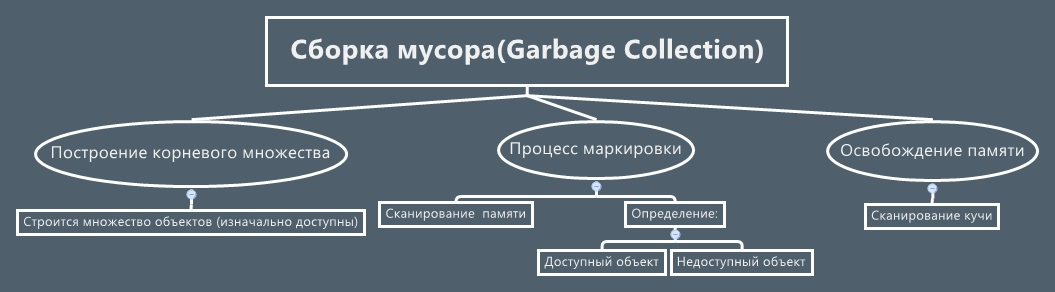
\includegraphics[width=500pt]{picture1.jpg}
	\caption{Три основных этапа сборки мусора}
	\centering
\end{figure}

Алгоритм ``пометки и освобождения'' состоит из двух фаз, которые запускаются последовательно
одна за другой:

\begin{itemize}
\item Фаза пометки. Начиная с некоторого аксиоматически заданного множества указателей, называемого
\emph{корневым множеством}, происходит полный обход всех достижимых объектов. Каждый достижимый
объект помечается как живой.
\item Фаза освобождения. Происходит полный обход кучи, во время которого освобождается память
из-подо всех непомеченных объектов; при этом пометка с помеченых объектов снимается.
\end{itemize}

Для реализации сборки мусора с помощью алгоритма ``пометки и освобождения'' должны быть решены
следующие задачи:

\begin{enumerate}
\item Идентификация корневого множества. Корневое множество~--- это множество указателей на
объекты, которые считаются изначально доступными для программы. Такие указатели хранятся в
стеке, регистрах и статической области памяти. В задачу идентификации корневого множества 
входит распознавание указателей в кучу на отведенные там объекты среди всех таких значений.

\item Определение всех ссылок из данного объекта на другие объекты в куче, что необходимо для
обхода всех достижимых объектов в фазе пометки.

\item Обеспечение возможности пометки объектов в куче и обхода всей кучи с освобождением 
непомеченных объектов.
\end{enumerate}

Последняя задача относится к реализации кучи; её решение изложено в~\cite{realisation}. Ниже 
мы опишем, как с помощью пользовательских примитивов, введенных в предыдущем разделе,
нами решаются две первые задачи.

\subsection{Поддержка корневого множества}

Идентификация корневого множества указателей (то есть указателей, хранящихся на стеке, в регистрах и статической
области памяти) без помощи со стороны компилятора является серьезной проблемой~\cite{roots}. При ``библиотечном''
подходе к сборке мусора рассчитывать на поддержку со стороны компилятора не приходится, поэтому в момент
начала сборки мусора идентифицировать корневые указатели уже невозможно. Поэтому корневое множество
поддерживается по мере работы программы. В него добавляются все \lstinline{gc_ptr}, экземпляры которых
не созданы с помощью \lstinline{gc_new}. Для этого в функции \lstinline{gc_new} выставляется флаг,
который проверяется в конструкторе \lstinline{gc_ptr}; в этом же конструкторе происходит добавление
указателя на объект \lstinline{gc_ptr} в пул корней, если это необходимо. Удаление же корневого
указателя происходит при вызове его деструктора. Так как удалять нужно только корневые указатели, а деструкторы
вызываются для всех, в \lstinline{gc_ptr} хранится признак того, что это корень. Поскольку деструкторы 
вызывается по отношению к конструкторам в обратном порядке (для автоматических объектов), пул корней можно 
реализовать в виде стека в отдельной области памяти вне кучи. 

\subsection{Построение метаинформации}

Представление метаинформации для сборки мусора, использованное нами, близко к тому, что описано
в~\cite{meta}. Метаинформация для типа представляет собой вектор смещений объектов \lstinline{gc_ptr} 
относительно начала экземпляра этого типа. Функция \lstinline{gc_new}, используемая для создания объектов, 
осуществляет поиск метаинформации по имени типа, полученному с помощью функции \lstinline{typeid}. 
Если этот поиск неуспешен (и, следовательно, для данного типа еще не была построена метаинформация), 
то создается новый объект, хранящий метаинформацию, и ассоциируется с именем этого типа. Для построения
метаинформации используются вызовы конструкторов \lstinline{gc_ptr}, с помощью которых можно
посчитать разность между адресом начала объекта и адресом, по которому ``внутри'' него расположен данный
\lstinline{gc_ptr}. 

После получения метаинформации функция \lstinline{gc_new} размещает указатель на неё перед данными 
создаваемого объекта. Это даёт возможность по указателю на живой объект узнать все указатели
из него на другие живые объекты, то есть реализовать стадию маркировки.

\newpage
\section{Заключение}

В результате выполнения данной дипломной работы были достигнуты следующие результаты:

\begin{enumerate}
\item изучены различные способы автоматизации управления памятью для языка C++ на 
основе использования ``умных указателей'';

\item разработан интерфейс библиотеки, позволяющей реализовать неконсервативную сборку мусора
при выполнении определенных соглашений на вид использующей её программы.

\item данное решение было использовано в рамках проекта по разработке библиотеки неконсервативной 
сборки мусора для языка С++;

\item полученная библиотека была протестирована на ряде примеров.
\end{enumerate}

%\newpage
\bibliographystyle{plainnat}
\addcontentsline{toc}{section}{Список литературы}
\begin{thebibliography}{}

\bibitem{GCBook} 
Richard Jones, Rafael Lins. Garbage Collection: Algorithms for Automatic Dynamic Memory Management. John Wiley \& Sons, 2001.

\bibitem{roots}
Д.А. Березун. Построение корневого множества указателей для сборки мусора // Труды лаборатории языковых инструментов JetBrains, 
выпуск 1. Санкт-Петербург, 2013.

\bibitem{meta}
М.В. Крень. Представление данных для сборки мусора // Труды лаборатории языковых инструментов JetBrains, выпуск 1. Санкт-Петербург, 2013.


\bibitem{realisation}
Д.А. Березун. Реализация основных примитивов библиотеки неконсервативной сборки мусора для С++. Дипломная работа, СПбГУ, 2014.


\bibitem{standart}
Bjarne Stroustrup. C++11 --- the new ISO C++ standard // \url{http://www.stroustrup.com/C++11FAQ.html}


\end{thebibliography}

%\newpage
%\appendix

\section{Программный код полиномиальной сложности оптимальных принтер-комбинаторов на языке Haskell}
\label{app:1}

\lstinputlisting[language=Haskell]{codes/PrettyLib.hs}


% \bibliographystyle{ugost2008ls}
% \bibliography{diploma.bib}

\end{document}
